\documentclass[11pt,a4paper]{article}

\usepackage[margin=1.05in]{geometry}
\usepackage[T1]{fontenc}
\usepackage{lmodern}
\usepackage{microtype}
\usepackage{amsmath,amssymb}
\usepackage{booktabs}
\usepackage{longtable}
\usepackage{graphicx}
\usepackage{xcolor}
\usepackage{natbib}
\usepackage{breakcites}   % long \citep{} groups may wrap
\usepackage{caption}
\usepackage[hidelinks,breaklinks=true]{hyperref}
\usepackage{enumitem}

\graphicspath{{../results/figures/}}
\captionsetup{font=small,labelfont=bf}
\setlist{itemsep=1pt,topsep=3pt}
% Prose carrying long \texttt{} paths and unbreakable \citep{} groups left five
% lines overfull -- the worst by 75pt, which is 26mm into the margin. Letting TeX
% loosen those lines is the right trade: a slightly wide word space is invisible,
% a line running off the page is not.
\setlength{\emergencystretch}{3em}
\bibliographystyle{plainnat}

% a Wilson interval, printed the same way everywhere
\newcommand{\ci}[2]{{\footnotesize\color{black!55}[#1,\,#2]}}
\newcommand{\defect}[1]{\textsc{#1}}
% generated by paper/build_tables.py -- do not edit
\newcommand{\numAlignAngle}{33.6}
\newcommand{\numAlignCos}{0.833}
\newcommand{\numAlignCubefrictionDown}{83.5}
\newcommand{\numAlignCubefrictionSigma}{174.0}
\newcommand{\numAlignCubefrictionTask}{6.8}
\newcommand{\numAlignCubefrictionUp}{86.5}
\newcommand{\numAlignCubemassDown}{84.5}
\newcommand{\numAlignCubemassSigma}{65.6}
\newcommand{\numAlignCubemassTask}{9.1}
\newcommand{\numAlignCubemassUp}{88.5}
\newcommand{\numAlignJointdampingDown}{85.5}
\newcommand{\numAlignJointdampingSigma}{29.5}
\newcommand{\numAlignJointdampingTask}{0.0}
\newcommand{\numAlignJointdampingUp}{85.5}
\newcommand{\numCollateralMax}{29.4}
\newcommand{\numDirectClutClean}{79.3}
\newcommand{\numDirectClutCleanHi}{83.5}
\newcommand{\numDirectClutCleanLo}{74.4}
\newcommand{\numDirectClutN}{300}
\newcommand{\numDirectClutNOcc}{124}
\newcommand{\numDirectClutOcc}{55.6}
\newcommand{\numDirectClutOccHi}{64.1}
\newcommand{\numDirectClutOccLo}{46.9}
\newcommand{\numDirectClutSecs}{0.38}
\newcommand{\numDirectClutSeedHi}{82.7}
\newcommand{\numDirectClutSeedLo}{76.0}
\newcommand{\numDirectClutSims}{0.00}
\newcommand{\numDirectOpenClean}{88.3}
\newcommand{\numDirectOpenCleanHi}{91.5}
\newcommand{\numDirectOpenCleanLo}{84.2}
\newcommand{\numDirectOpenN}{300}
\newcommand{\numDirectOpenNOcc}{105}
\newcommand{\numDirectOpenOcc}{66.7}
\newcommand{\numDirectOpenOccHi}{75.0}
\newcommand{\numDirectOpenOccLo}{57.2}
\newcommand{\numDirectOpenSecs}{0.33}
\newcommand{\numDirectOpenSeedHi}{92.0}
\newcommand{\numDirectOpenSeedLo}{81.3}
\newcommand{\numDirectOpenSims}{0.00}
\newcommand{\numFacExactBlind}{85.3}
\newcommand{\numFacExactBlindAgree}{86.7}
\newcommand{\numFacExactBlindFalse}{12.7}
\newcommand{\numFacExactBlindHi}{88.9}
\newcommand{\numFacExactBlindLo}{80.9}
\newcommand{\numFacExactBlindTwoStep}{17.0}
\newcommand{\numFacExactSeen}{90.7}
\newcommand{\numFacExactSeenAgree}{93.0}
\newcommand{\numFacExactSeenFalse}{6.3}
\newcommand{\numFacExactSeenHi}{93.5}
\newcommand{\numFacExactSeenLo}{86.8}
\newcommand{\numFacExactSeenTwoStep}{18.7}
\newcommand{\numFacNone}{79.3}
\newcommand{\numFacNoneAgree}{--}
\newcommand{\numFacNoneFalse}{--}
\newcommand{\numFacNoneHi}{83.5}
\newcommand{\numFacNoneLo}{74.4}
\newcommand{\numFacNoneTwoStep}{0.0}
\newcommand{\numFacPairedDirectnotwinBroke}{20}
\newcommand{\numFacPairedDirectnotwinP}{0.0001}
\newcommand{\numFacPairedDirectnotwinResc}{2}
\newcommand{\numFacPairedExactphysicsyawknoBroke}{7}
\newcommand{\numFacPairedExactphysicsyawknoP}{0.005}
\newcommand{\numFacPairedExactphysicsyawknoResc}{23}
\newcommand{\numFacPairedMisspecifiedyawknoBroke}{10}
\newcommand{\numFacPairedMisspecifiedyawknoP}{0.017}
\newcommand{\numFacPairedMisspecifiedyawknoResc}{25}
\newcommand{\numFacPairedMisspecifiedyawunsBroke}{1}
\newcommand{\numFacPairedMisspecifiedyawunsP}{0.0003}
\newcommand{\numFacPairedMisspecifiedyawunsResc}{16}
\newcommand{\numFacWrongBlind}{90.3}
\newcommand{\numFacWrongBlindAgree}{91.3}
\newcommand{\numFacWrongBlindFalse}{7.3}
\newcommand{\numFacWrongBlindHi}{93.2}
\newcommand{\numFacWrongBlindLo}{86.5}
\newcommand{\numFacWrongBlindTwoStep}{19.7}
\newcommand{\numFacWrongSeen}{90.3}
\newcommand{\numFacWrongSeenAgree}{94.0}
\newcommand{\numFacWrongSeenFalse}{5.7}
\newcommand{\numFacWrongSeenHi}{93.2}
\newcommand{\numFacWrongSeenLo}{86.5}
\newcommand{\numFacWrongSeenTwoStep}{18.3}
\newcommand{\numFixedActual}{79.3}
\newcommand{\numFixedN}{300}
\newcommand{\numIdentRank}{cube friction, cube mass, joint damping}
\newcommand{\numJudgeCameraMiss}{8}
\newcommand{\numJudgeCameraPrec}{100.0}
\newcommand{\numJudgeCameraPrecLo}{99.8}
\newcommand{\numJudgeCameraSaid}{1{,}599}
\newcommand{\numJudgeCameraWrong}{0}
\newcommand{\numJudgeSkillMiss}{8}
\newcommand{\numJudgeSkillPrec}{94.4}
\newcommand{\numJudgeSkillPrecLo}{93.3}
\newcommand{\numJudgeSkillSaid}{1{,}693}
\newcommand{\numJudgeSkillWrong}{94}
\newcommand{\numJudgeTwinMiss}{6}
\newcommand{\numJudgeTwinPrec}{93.0}
\newcommand{\numJudgeTwinPrecLo}{91.4}
\newcommand{\numJudgeTwinSaid}{1{,}181}
\newcommand{\numJudgeTwinWrong}{83}
\newcommand{\numLoopClutClean}{90.3}
\newcommand{\numLoopClutCleanHi}{93.2}
\newcommand{\numLoopClutCleanLo}{86.5}
\newcommand{\numLoopClutN}{300}
\newcommand{\numLoopClutNOcc}{124}
\newcommand{\numLoopClutOcc}{80.6}
\newcommand{\numLoopClutOccHi}{86.6}
\newcommand{\numLoopClutOccLo}{72.8}
\newcommand{\numLoopClutSecs}{0.77}
\newcommand{\numLoopClutSeedHi}{93.3}
\newcommand{\numLoopClutSeedLo}{86.7}
\newcommand{\numLoopClutSims}{1.28}
\newcommand{\numLoopExactClutClean}{85.3}
\newcommand{\numLoopExactClutCleanHi}{88.9}
\newcommand{\numLoopExactClutCleanLo}{80.9}
\newcommand{\numLoopExactClutN}{300}
\newcommand{\numLoopExactClutNOcc}{124}
\newcommand{\numLoopExactClutOcc}{68.5}
\newcommand{\numLoopExactClutOccHi}{76.1}
\newcommand{\numLoopExactClutOccLo}{59.9}
\newcommand{\numLoopExactClutSecs}{0.74}
\newcommand{\numLoopExactClutSeedHi}{89.3}
\newcommand{\numLoopExactClutSeedLo}{81.3}
\newcommand{\numLoopExactClutSims}{1.23}
\newcommand{\numLoopExactOpenClean}{95.7}
\newcommand{\numLoopExactOpenCleanHi}{97.5}
\newcommand{\numLoopExactOpenCleanLo}{92.7}
\newcommand{\numLoopExactOpenN}{300}
\newcommand{\numLoopExactOpenNOcc}{105}
\newcommand{\numLoopExactOpenOcc}{87.6}
\newcommand{\numLoopExactOpenOccHi}{92.6}
\newcommand{\numLoopExactOpenOccLo}{80.0}
\newcommand{\numLoopExactOpenSecs}{0.53}
\newcommand{\numLoopExactOpenSeedHi}{97.3}
\newcommand{\numLoopExactOpenSeedLo}{93.3}
\newcommand{\numLoopExactOpenSims}{1.17}
\newcommand{\numLoopOpenClean}{96.7}
\newcommand{\numLoopOpenCleanHi}{98.2}
\newcommand{\numLoopOpenCleanLo}{94.0}
\newcommand{\numLoopOpenN}{300}
\newcommand{\numLoopOpenNOcc}{105}
\newcommand{\numLoopOpenOcc}{90.5}
\newcommand{\numLoopOpenOccHi}{94.7}
\newcommand{\numLoopOpenOccLo}{83.4}
\newcommand{\numLoopOpenSecs}{0.55}
\newcommand{\numLoopOpenSeedHi}{100.0}
\newcommand{\numLoopOpenSeedLo}{89.3}
\newcommand{\numLoopOpenSims}{1.20}
\newcommand{\numPairedExactLoopClutteredBroke}{16}
\newcommand{\numPairedExactLoopClutteredP}{0.0003}
\newcommand{\numPairedExactLoopClutteredResc}{1}
\newcommand{\numPairedExactLoopOpenBroke}{6}
\newcommand{\numPairedExactLoopOpenP}{0.508}
\newcommand{\numPairedExactLoopOpenResc}{3}
\newcommand{\numPairedLoopDirectClutteredBroke}{1}
\newcommand{\numPairedLoopDirectClutteredP}{2\times 10^{-9}}
\newcommand{\numPairedLoopDirectClutteredResc}{34}
\newcommand{\numPairedLoopDirectOpenBroke}{0}
\newcommand{\numPairedLoopDirectOpenP}{6\times 10^{-8}}
\newcommand{\numPairedLoopDirectOpenResc}{25}
\newcommand{\numRepairClearthenplaceClut}{94.9}
\newcommand{\numRepairClearthenplaceClutHi}{98.3}
\newcommand{\numRepairClearthenplaceClutLo}{86.1}
\newcommand{\numRepairClearthenplaceClutN}{59}
\newcommand{\numRepairClearthenplaceOpen}{100.0}
\newcommand{\numRepairClearthenplaceOpenHi}{100.0}
\newcommand{\numRepairClearthenplaceOpenLo}{94.1}
\newcommand{\numRepairClearthenplaceOpenN}{61}
\newcommand{\numRepairDirectClut}{89.8}
\newcommand{\numRepairDirectClutHi}{93.1}
\newcommand{\numRepairDirectClutLo}{85.3}
\newcommand{\numRepairDirectClutN}{236}
\newcommand{\numRepairDirectOpen}{95.8}
\newcommand{\numRepairDirectOpenHi}{97.7}
\newcommand{\numRepairDirectOpenLo}{92.5}
\newcommand{\numRepairDirectOpenN}{239}
\newcommand{\numRepairTurnwristClut}{60.0}
\newcommand{\numRepairTurnwristClutHi}{88.2}
\newcommand{\numRepairTurnwristClutLo}{23.1}
\newcommand{\numRepairTurnwristClutN}{5}
\newcommand{\numSelLoopClutCov}{96.3}
\newcommand{\numSelLoopClutEnd}{92.4}
\newcommand{\numSelLoopClutEndHi}{94.9}
\newcommand{\numSelLoopClutEndLo}{88.7}
\newcommand{\numSelLoopClutNUn}{11}
\newcommand{\numSelLoopClutUn}{36.4}
\newcommand{\numSelLoopClutUnHi}{64.6}
\newcommand{\numSelLoopClutUnLo}{15.2}
\newcommand{\numSelLoopExactClutCov}{97.3}
\newcommand{\numSelLoopExactClutEnd}{87.0}
\newcommand{\numSelLoopExactClutEndHi}{90.4}
\newcommand{\numSelLoopExactClutEndLo}{82.6}
\newcommand{\numSelLoopExactClutNUn}{8}
\newcommand{\numSelLoopExactClutUn}{25.0}
\newcommand{\numSelLoopExactClutUnHi}{59.1}
\newcommand{\numSelLoopExactClutUnLo}{7.1}
\newcommand{\numSelLoopExactOpenCov}{100.0}
\newcommand{\numSelLoopExactOpenEnd}{95.7}
\newcommand{\numSelLoopExactOpenEndHi}{97.5}
\newcommand{\numSelLoopExactOpenEndLo}{92.7}
\newcommand{\numSelLoopExactOpenNUn}{0}
\newcommand{\numSelLoopOpenCov}{100.0}
\newcommand{\numSelLoopOpenEnd}{96.7}
\newcommand{\numSelLoopOpenEndHi}{98.2}
\newcommand{\numSelLoopOpenEndLo}{94.0}
\newcommand{\numSelLoopOpenNUn}{0}
\newcommand{\numSelPoolCov}{98.4}
\newcommand{\numSelPoolEnd}{93.0}
\newcommand{\numSelPoolEndHi}{94.3}
\newcommand{\numSelPoolEndLo}{91.4}
\newcommand{\numSelPoolNUn}{19}
\newcommand{\numSelPoolUn}{31.6}
\newcommand{\numSelPoolUnHi}{54.0}
\newcommand{\numSelPoolUnLo}{15.4}
\newcommand{\numSigmaCube}{1.7}
\newcommand{\numSigmaJoint}{1.0}
\newcommand{\numSweepMinusHalf}{87.3}
\newcommand{\numSweepMinusHalfAcc}{79.0}
\newcommand{\numSweepMinusHalfAccHi}{83.2}
\newcommand{\numSweepMinusHalfAccLo}{74.0}
\newcommand{\numSweepMinusHalfBroke}{3}
\newcommand{\numSweepMinusHalfFalse}{10.7}
\newcommand{\numSweepMinusHalfHi}{90.6}
\newcommand{\numSweepMinusHalfLo}{83.1}
\newcommand{\numSweepMinusHalfP}{0.146}
\newcommand{\numSweepMinusHalfPred}{79.7}
\newcommand{\numSweepMinusHalfResc}{9}
\newcommand{\numSweepMinusOne}{88.3}
\newcommand{\numSweepMinusOneAcc}{81.0}
\newcommand{\numSweepMinusOneAccHi}{85.0}
\newcommand{\numSweepMinusOneAccLo}{76.2}
\newcommand{\numSweepMinusOneBroke}{5}
\newcommand{\numSweepMinusOneFalse}{9.0}
\newcommand{\numSweepMinusOneHi}{91.5}
\newcommand{\numSweepMinusOneLo}{84.2}
\newcommand{\numSweepMinusOneP}{0.064}
\newcommand{\numSweepMinusOnePred}{78.3}
\newcommand{\numSweepMinusOneResc}{14}
\newcommand{\numSweepMinusThree}{84.3}
\newcommand{\numSweepMinusThreeAcc}{83.3}
\newcommand{\numSweepMinusThreeAccHi}{87.1}
\newcommand{\numSweepMinusThreeAccLo}{78.7}
\newcommand{\numSweepMinusThreeBroke}{11}
\newcommand{\numSweepMinusThreeFalse}{13.0}
\newcommand{\numSweepMinusThreeHi}{88.0}
\newcommand{\numSweepMinusThreeLo}{79.8}
\newcommand{\numSweepMinusThreeP}{0.648}
\newcommand{\numSweepMinusThreePred}{88.7}
\newcommand{\numSweepMinusThreeResc}{8}
\newcommand{\numSweepMinusTwo}{86.7}
\newcommand{\numSweepMinusTwoAcc}{84.0}
\newcommand{\numSweepMinusTwoAccHi}{87.7}
\newcommand{\numSweepMinusTwoAccLo}{79.4}
\newcommand{\numSweepMinusTwoBroke}{7}
\newcommand{\numSweepMinusTwoFalse}{10.3}
\newcommand{\numSweepMinusTwoHi}{90.1}
\newcommand{\numSweepMinusTwoLo}{82.4}
\newcommand{\numSweepMinusTwoP}{0.481}
\newcommand{\numSweepMinusTwoPred}{84.0}
\newcommand{\numSweepMinusTwoResc}{11}
\newcommand{\numSweepPlusHalf}{87.0}
\newcommand{\numSweepPlusHalfAcc}{77.3}
\newcommand{\numSweepPlusHalfAccHi}{81.7}
\newcommand{\numSweepPlusHalfAccLo}{72.3}
\newcommand{\numSweepPlusHalfBroke}{3}
\newcommand{\numSweepPlusHalfFalse}{10.3}
\newcommand{\numSweepPlusHalfHi}{90.3}
\newcommand{\numSweepPlusHalfLo}{82.7}
\newcommand{\numSweepPlusHalfP}{0.227}
\newcommand{\numSweepPlusHalfPred}{77.3}
\newcommand{\numSweepPlusHalfResc}{8}
\newcommand{\numSweepPlusOne}{90.3}
\newcommand{\numSweepPlusOneAcc}{84.0}
\newcommand{\numSweepPlusOneAccHi}{87.7}
\newcommand{\numSweepPlusOneAccLo}{79.4}
\newcommand{\numSweepPlusOneBroke}{1}
\newcommand{\numSweepPlusOneFalse}{7.0}
\newcommand{\numSweepPlusOneHi}{93.2}
\newcommand{\numSweepPlusOneLo}{86.5}
\newcommand{\numSweepPlusOneP}{0.0003}
\newcommand{\numSweepPlusOnePred}{77.3}
\newcommand{\numSweepPlusOneResc}{16}
\newcommand{\numSweepPlusThree}{90.0}
\newcommand{\numSweepPlusThreeAcc}{81.3}
\newcommand{\numSweepPlusThreeAccHi}{85.3}
\newcommand{\numSweepPlusThreeAccLo}{76.5}
\newcommand{\numSweepPlusThreeBroke}{9}
\newcommand{\numSweepPlusThreeFalse}{7.3}
\newcommand{\numSweepPlusThreeHi}{92.9}
\newcommand{\numSweepPlusThreeLo}{86.1}
\newcommand{\numSweepPlusThreeP}{0.020}
\newcommand{\numSweepPlusThreePred}{75.3}
\newcommand{\numSweepPlusThreeResc}{23}
\newcommand{\numSweepPlusTwo}{89.0}
\newcommand{\numSweepPlusTwoAcc}{84.7}
\newcommand{\numSweepPlusTwoAccHi}{88.3}
\newcommand{\numSweepPlusTwoAccLo}{80.2}
\newcommand{\numSweepPlusTwoBroke}{7}
\newcommand{\numSweepPlusTwoFalse}{7.7}
\newcommand{\numSweepPlusTwoHi}{92.1}
\newcommand{\numSweepPlusTwoLo}{85.0}
\newcommand{\numSweepPlusTwoP}{0.043}
\newcommand{\numSweepPlusTwoPred}{79.3}
\newcommand{\numSweepPlusTwoResc}{18}
\newcommand{\numSweepZero}{85.3}
\newcommand{\numSweepZeroAcc}{78.0}
\newcommand{\numSweepZeroAccHi}{82.3}
\newcommand{\numSweepZeroAccLo}{73.0}
\newcommand{\numSweepZeroFalse}{12.0}
\newcommand{\numSweepZeroHi}{88.9}
\newcommand{\numSweepZeroLo}{80.9}
\newcommand{\numSweepZeroPred}{81.3}
\newcommand{\numTauFifteenClutBroke}{1}
\newcommand{\numTauFifteenClutDirect}{77.3}
\newcommand{\numTauFifteenClutLoop}{87.7}
\newcommand{\numTauFifteenClutP}{8\times 10^{-9}}
\newcommand{\numTauFifteenClutResc}{32}
\newcommand{\numTauFifteenOpenBroke}{0}
\newcommand{\numTauFifteenOpenDirect}{88.3}
\newcommand{\numTauFifteenOpenLoop}{96.7}
\newcommand{\numTauFifteenOpenP}{6\times 10^{-8}}
\newcommand{\numTauFifteenOpenResc}{25}
\newcommand{\numTauFiftyClutBroke}{1}
\newcommand{\numTauFiftyClutDirect}{79.3}
\newcommand{\numTauFiftyClutLoop}{90.3}
\newcommand{\numTauFiftyClutP}{2\times 10^{-9}}
\newcommand{\numTauFiftyClutResc}{34}
\newcommand{\numTauFiftyOpenBroke}{0}
\newcommand{\numTauFiftyOpenDirect}{88.3}
\newcommand{\numTauFiftyOpenLoop}{96.7}
\newcommand{\numTauFiftyOpenP}{6\times 10^{-8}}
\newcommand{\numTauFiftyOpenResc}{25}
\newcommand{\numTauTenClutBroke}{1}
\newcommand{\numTauTenClutDirect}{76.7}
\newcommand{\numTauTenClutLoop}{86.7}
\newcommand{\numTauTenClutP}{2\times 10^{-8}}
\newcommand{\numTauTenClutResc}{31}
\newcommand{\numTauTenOpenBroke}{0}
\newcommand{\numTauTenOpenDirect}{88.0}
\newcommand{\numTauTenOpenLoop}{96.3}
\newcommand{\numTauTenOpenP}{6\times 10^{-8}}
\newcommand{\numTauTenOpenResc}{25}
\newcommand{\numTauThirtyClutBroke}{1}
\newcommand{\numTauThirtyClutDirect}{79.3}
\newcommand{\numTauThirtyClutLoop}{90.3}
\newcommand{\numTauThirtyClutP}{2\times 10^{-9}}
\newcommand{\numTauThirtyClutResc}{34}
\newcommand{\numTauThirtyOpenBroke}{0}
\newcommand{\numTauThirtyOpenDirect}{88.3}
\newcommand{\numTauThirtyOpenLoop}{96.7}
\newcommand{\numTauThirtyOpenP}{6\times 10^{-8}}
\newcommand{\numTauThirtyOpenResc}{25}
\newcommand{\numTauTwentyClutBroke}{1}
\newcommand{\numTauTwentyClutDirect}{78.0}
\newcommand{\numTauTwentyClutLoop}{88.7}
\newcommand{\numTauTwentyClutP}{4\times 10^{-9}}
\newcommand{\numTauTwentyClutResc}{33}
\newcommand{\numTauTwentyOpenBroke}{0}
\newcommand{\numTauTwentyOpenDirect}{88.3}
\newcommand{\numTauTwentyOpenLoop}{96.7}
\newcommand{\numTauTwentyOpenP}{6\times 10^{-8}}
\newcommand{\numTauTwentyOpenResc}{25}
\newcommand{\numTaxCollateralTotal}{0}
\newcommand{\numTaxSilentTotal}{94}


\title{\bfseries The best twin is not the true one:\\[2pt]
       \large fidelity, identifiability and verification in a\\
       simulate-before-acting tabletop manipulator}

\author{Samjhana Bhusal\thanks{Correspondence via the repository accompanying
this report. Code, raw results and a reproduction command for every figure and
table are in \texttt{README.md}.}}

\date{November 2026}

\begin{document}
\maketitle

\begin{abstract}
\noindent
A robot that rolls its plan out in a digital twin before committing to it needs
an answer to a question the digital-twin literature mostly assumes: how accurate
does the twin have to be? We build a language-commanded tabletop manipulator in
MuJoCo that looks at the scene through its own overhead camera, plans, simulates
the plan in a deliberately mis-specified twin, repairs the plan if the twin
predicts failure, executes, and then verifies the outcome from a second
photograph. Over 1{,}800 paired episodes the loop lifts clean task success from
\numDirectOpenClean\% to \numLoopOpenClean\% in an open scene and from
\numDirectClutClean\% to \numLoopClutClean\% in clutter, with the gain
concentrated in the task class that cannot be completed by a single
pick-and-place. We then sweep the twin's mis-specification through zero and out
the other side, as a signed magnitude in log-parameter space. The twin holding
the plant's \emph{true} parameters is the minimum of both curves: it is neither
the most useful (\numSweepZero\% against \numSweepPlusOne\%) nor, measured on a
plan it did not itself choose, the most accurate (\numSweepZeroAcc\% against
\numSweepPlusTwoAcc\%). A $2\times2$ explains why. The twin's two ignorances ---
wrong physics, and blindness to how objects are oriented --- are
\emph{substitutes} rather than additive, and the dominant one is the geometry,
not the physics. Parameter error that happens to be pessimistic cancels the
optimism caused by the unseen orientation, and buys exactly what seeing the
orientation would have bought and no more. Two further results follow. Overall
predictive agreement is the wrong score for a twin, because a twin can buy it by
agreeing with the common case while carrying the highest false confidence in the
sweep; what matters is being right about the failures. And the parameter a
scripted push identifies best is not the parameter the task is most sensitive to
--- the top two are swapped, and a third parameter is cleanly identifiable and
worth nothing at all. We report the instrument's own defects alongside its
results, including a ceiling effect, a seven-point seed artefact, a
configuration flag that was silently inert, and an endogenous accuracy metric,
each with the measurement that exposed it. The study is simulation-only; no
claim of real-robot transfer is made or tested.
\end{abstract}

\section{Introduction}

A manipulator that is about to act can, in principle, check first. If a
sufficiently faithful model of the scene is available, the robot can roll its
intended plan out in that model, look at what happens, and revise the plan
before anything in the world has moved. This is the operational promise of the
digital twin \citep{grieves2017digital,jones2020characterising}, and on a
tabletop with a fast rigid-body simulator it is not expensive: an episode here
costs a fraction of a second, so simulating one before executing it roughly
doubles the cost of an action that was already cheap.

The promise comes with an obvious objection. The twin is a model, and models are
wrong. The literature on crossing that gap is large and almost entirely
concerned with making the model \emph{less} wrong --- by identifying its
parameters from data \citep{gautier1992exciting,swevers2007dynamic}, by adapting
a randomisation distribution towards reality \citep{chebotar2019closing,
ramos2019bayessim}, or by training policies that tolerate the residual
\citep{tobin2017domain,peng2018sim,muratore2022robot}. Comparatively little of
it asks the question an engineer with a fixed budget actually faces: \emph{how
accurate does the model have to be before the rollout is worth running?} and,
sharper, \emph{is accuracy even the right axis?}

This report answers both on one small system, measured rather than argued. We
build a language-commanded tabletop manipulator --- a Franka Panda in MuJoCo
\citep{todorov2012mujoco} --- that executes instructions like \emph{``put the red
cube where the blue cube is''}. It looks at the table through its own overhead
camera, grounds the instruction onto an object, builds a plan, rolls the plan out
in a twin, repairs the plan if the twin predicts failure, executes, and then
verifies the outcome from a second photograph. The twin is wrong on purpose and
in two separable ways: its object positions come from the camera rather than from
simulator state, and its mass, friction and damping parameters are offset by a
controlled amount. Making the twin wrong is not a flourish. MuJoCo is
deterministic, so a twin that is an exact copy of the plant handed an identical
state and an identical control sequence reproduces the plant exactly, and the
question ``did the twin predict the outcome?'' answers itself.

\paragraph{Contributions.}
\begin{enumerate}[leftmargin=1.4em]
\item \textbf{The loop pays, and we show where.} Simulate-repair-execute lifts
clean success from \numDirectOpenClean\% to \numLoopOpenClean\% (open) and
\numDirectClutClean\% to \numLoopClutClean\% (cluttered) over 1{,}800 paired
episodes, at a mean of \numLoopClutSims\ simulated rollouts per episode. The gain
is concentrated in occupied-destination tasks, which rise from
\numDirectClutOcc\% to \numLoopClutOcc\%.
\item \textbf{Twin fidelity is not monotone in twin usefulness.} Swept as a
signed magnitude, the twin with the plant's true parameters is the
\emph{minimum} of both the usefulness and the accuracy curve
(Section~\ref{sec:sweep}).
\item \textbf{We explain the non-monotonicity rather than reporting it.} A
$2\times2$ crossing wrong physics against unseen orientation shows the two
ignorances to be substitutes, and identifies the geometric one as dominant
(Section~\ref{sec:factorial}).
\item \textbf{Overall agreement is the wrong score for a twin.} Measured on a
fixed plan no twin chose, the most optimistic twin matches the best twin on
agreement while being the worst arm to plan with, because its errors are all
false confidence (Section~\ref{sec:fixedplan}).
\item \textbf{Identifiability and task sensitivity disagree on the same
system.} Over three parameters in one set of units, the identification ranking
and the task ranking swap their top two, and a cleanly identifiable parameter
turns out to be worth nothing (Section~\ref{sec:alignment}).
\item \textbf{The loop yields a usable abstention signal for free.} A plan the
twin never endorsed within its budget is clean \numSelPoolUn\% of the time
against \numSelPoolEnd\% for endorsed plans, at \numSelPoolCov\% coverage
(Section~\ref{sec:selective}).
\item \textbf{We report the instrument's defects as results.} Section~\ref{sec:defects}
tabulates eight, each with the measurement that exposed it and what it cost.
\end{enumerate}

\paragraph{What this is not.} Everything here runs in simulation. No claim is
made that these numbers transfer to hardware, and the central result --- that a
pessimistically wrong twin beats an exact one --- is a statement about a
\emph{twin of a simulator}, where ``exact'' is achievable and therefore
measurable. On hardware it is not achievable, which is what makes the simulated
version of the question answerable at all; whether the shape of the curve
survives the transfer is untested and we flag it as the principal threat to
validity in Section~\ref{sec:limits}.

\section{Related work}

\subsection{Digital twins}
The digital twin is usually characterised as a virtual counterpart kept in
correspondence with a physical asset, used for monitoring, prediction and
control \citep{grieves2017digital,tao2019digital}. A systematic review of 92
publications \citep{jones2020characterising} consolidates the concept into
thirteen characteristics and explicitly lists \emph{levels of fidelity} among its
open knowledge gaps --- the question of how good the correspondence must be is
named as unresolved rather than answered. Most robotics work invoking the term
uses the twin for monitoring or for offline optimisation. We use it inside the
control loop, as a veto on a plan about to be executed, which makes the fidelity
question immediate rather than architectural: a rollout that is not predictive
is not merely imprecise, it actively licenses the wrong action.

\subsection{The reality gap, and model error introduced on purpose}
Domain randomisation \citep{tobin2017domain,peng2018sim} makes a policy robust by
training it across a distribution of models rather than one, and is now
surveyed as a field in its own right \citep{muratore2022robot}. Later work closes
the loop by adapting the randomisation distribution towards real data
\citep{chebotar2019closing,ramos2019bayessim}. The closest antecedent to our
central result is not in that line but in planning: \citet{mordatch2015ensemble}
found that trajectories optimised against a \emph{single} accurate model of a
humanoid did not transfer, and that planning across an ensemble of perturbed
models did, because a plan that survives several models does not depend on the
details of any one of them. \citet{rajeswaran2017epopt} make the same move for
policy search with a risk-sensitive objective over a model ensemble.

Our finding is that effect at an ensemble size of one, and with an added twist
those papers do not report: the perturbation's \emph{sign} matters.
Section~\ref{sec:sweep} sweeps the mis-specification through zero and out the
other side, and the two sides are not equivalent. A twin biased towards
expecting failure is useful; its exact mirror, biased towards expecting success,
is the worst arm measured. Ensemble methods average over perturbations and
therefore cannot see this asymmetry; a single biased model can.

\subsection{Model error measured against a decision rather than against data}
The observation that predictive accuracy and downstream usefulness come apart is
well established in model-based reinforcement learning, where it is called
objective mismatch: a dynamics model trained to maximise one-step likelihood is
not thereby trained to produce good control, and the two are empirically
uncorrelated over much of the training run \citep{lambert2020objective}.
Responses include learning models that are equivalent only with respect to the
values they induce \citep{grimm2020value,farahmand2018iterative}, and, in
operations research, training predictors against the decision loss they feed
\citep{donti2017task,elmachtoub2022smart}.

That literature establishes that accuracy and usefulness are \emph{different}.
What we add is a case where they are \emph{anti-correlated in a specific and
diagnosable region}: not merely that the most accurate model fails to be the
most useful, but that the exactly correct model is the worst of nine, and that
the mechanism --- an unmodelled state variable that biases the model
optimistically, cancelled by parameter error biased the other way --- can be
isolated by a factorial and confirmed by its saturation point.

\subsection{World models and planning in a model}
Learned world models \citep{ha2018world,hafner2020dream,hafner2023mastering}
pursue the same structure we use --- imagine the consequences of an action
before taking it --- with the model learned rather than given. We use an
analytic twin instead, for a deliberate reason: the mis-specification has to be
a quantity we can set and sweep. A learned model is wrong in a way the
experimenter does not control, which makes it unsuitable as the independent
variable in the experiment this report is about. The classical planning
literature on deciding \emph{what} to do and \emph{how} to do it jointly
\citep{garrett2021integrated,kaelbling2013integrated} is where our plan
representation and repair catalogue sit; our planner is deliberately small, since
it is the instrument and not the subject.

\subsection{Identifiability and experiment design}
Robot parameter identification has a long tradition of designing excitation
trajectories to make parameters well conditioned
\citep{gautier1992exciting,swevers2007dynamic}, and optimal experiment design
formalises the choice \citep{pukelsheim1993optimal}. Those criteria are
properties of the identification problem --- how sharply the data constrains a
parameter. Section~\ref{sec:alignment} measures that criterion and the
\emph{task's} sensitivity to the same parameters in the same units, and finds
them misaligned by $\numAlignAngle^\circ$ with the top two ranks swapped. The
practical reading is that an identification budget spent where the data is most
informative is not thereby spent where the task is most sensitive.

\subsection{Knowing that something went wrong}
A skill that grasps, carries and releases cannot tell from inside whether the
task was accomplished. Recent work uses vision-language models as success
detectors \citep{du2023vision} and to explain failures after the fact
\citep{liu2023reflect}. Our verifier is deliberately not learned --- it is hue
segmentation and un-projection \citep{hartley2003multiple} --- which makes it the
baseline any future learned verifier in this system has to beat, and lets us
quantify the gap between what a skill believes and what a photograph shows
(Section~\ref{sec:judges}). Separately, the loop's own endorsement flag is an
abstention signal in the sense of selective classification
\citep{elyaniv2010foundations,geifman2017selective}, and we evaluate it as one.

A parallel line maps instructions and images directly onto actions, either by
scoring language-specified skills against learned affordances
\citep{ahn2022saycan} or by training a single vision-language-action model
end to end \citep{driess2023palme,brohan2023rt2,kim2024openvla}. We keep
language out of the control path on purpose. The question here is what the
\emph{rollout} is worth, and a learned policy that has absorbed the instruction,
the perception and the control into one set of weights makes that question
unaskable: there would be no plan to simulate and no separable model to
mis-specify.

\subsection{Benchmarking practice}
The methodology here follows the reproducibility literature in reinforcement
learning rather than the robotics benchmarking one. \citet{henderson2018deep} and
\citet{colas2018how} document how large seed variance is relative to reported
effects, and \citet{agarwal2021deep} argue for interval estimates and paired
aggregates over point estimates. Section~\ref{sec:defects} reports an instance
--- a seven-point swing in the headline rate produced by nothing but the seeding
scheme --- and the design change it forced. Tabletop manipulation benchmarks such
as RLBench \citep{james2020rlbench} and robosuite \citep{zhu2020robosuite} supply
task suites; we build a smaller one because we need to control the difficulty
dial precisely and to generate instructions with provable non-ambiguity.

\section{System}
\label{sec:system}

\subsection{Scene, robot and skills}
The scene is composed programmatically with MuJoCo's \texttt{MjSpec} API: a
Franka Panda loaded unmodified from MuJoCo Menagerie \citep{zakka2022menagerie}
via \texttt{robot\_descriptions}, a table, an overhead and a wrist camera, a
green pad and a vertical pipe as landmarks, and three or five coloured cubes.
Nothing from Menagerie is forked, so upstream fixes arrive for free. Cartesian
motion is differential inverse kinematics through mink \citep{zakka2024mink},
which poses each control step as a quadratic program --- frame task, posture
task, configuration limits --- solved with DAQP \citep{arnstrom2022daqp}.

Three skills are written here: \texttt{pick}, \texttt{place} and \texttt{push},
each with an approach/retreat structure and, more importantly, an explicit
success predicate. A skill returns a reason, never a bare boolean, because the
loop's repair selection is conditioned on \emph{how} a plan failed and not merely
that it did. ``Held'' is defined as both fingers in simultaneous contact with
the named body, read from MuJoCo's contact list. An earlier definition using the
finger gap plus the distance from the tool centre point to the object is
reported as defect~\defect{D8} in Section~\ref{sec:defects}.

\subsection{Perception}
The twin's input and the verifier's evidence are the same overhead image. Cubes
are segmented by hue and saturation and un-projected onto the table plane through
the pinhole model \citep{hartley2003multiple}, using the camera pose and field of
view the simulator reports. Hue rather than RGB, because the rendered image is
subject to specular wash-out that moves RGB far from the nominal colour while
leaving hue intact. The estimator locates every cube to a median error of
\numSigmaCube\,mm in 37\,ms, with no learned component. It reports position only:
a top-down blob of colour says nothing about which way a cube is turned, and that
omission turns out to be the most consequential fact about the whole system
(Section~\ref{sec:factorial}).

\subsection{Tasks}
A task is a \emph{reference} (which object the instruction is about) and a
\emph{goal} (a predicate on simulator state). The generator produces roughly 53
well-posed instructions per layout across five reference types --- colour,
nearest/farthest from a landmark, left/right of another cube, left/right of a
landmark, superlatives --- and five goal types. It refuses two kinds of bad
instruction: references whose runner-up is within 55\,mm, and goals already true
at the start. References are resolved from ground truth, so that when a
vision-language grounder replaces that step the drop is attributable to
grounding.

\subsection{Plans, repairs and the twin}
A plan is a short list of steps held as data rather than as control flow,
because it has to be handed to the twin and run there before it is handed to the
robot. The repair catalogue has four entries, each earned from a measured failure
mode: clear the blocker then place; re-aim to a different acceptable placement;
turn the wrist by $\pi/2$, which is the same grasp on the same faces of a
90$^\circ$-symmetric cube with the fingers arriving along the other axis; and
push instead of pick, where the goal's tolerance is loose enough to absorb a
push's imprecision.

One repair is deliberately absent. Shoving a neighbour aside to make room for the
fingers would fix the grasp and fail the episode on collateral damage. The
scoring rule, not taste, rules it out --- which is the clearest illustration we
have of a scoring rule doing design work.

The twin is a second MuJoCo model built from the same scene specification, then
mis-specified. \texttt{TwinFidelity} holds multipliers on cube mass, cube
friction and arm joint damping, plus a flag for whether the twin may be told the
true orientation of each cube. The multipliers are parameterised as a signed
magnitude $k$ along a unit direction in log-parameter space,
$\theta_{\text{twin}} = \theta \odot \exp(k\,\hat{u})$, so that $-1$ is the exact
mirror of $+1$ and a sweep through zero is one experiment rather than two. The
twin and the plant run \emph{the same plan-execution code}; nothing in that
function knows which world it is operating on, so any divergence comes from the
model and not from a second implementation.

\subsection{Verification}
After execution the robot parks, takes a second photograph, and re-evaluates the
goal predicate against estimated positions rather than simulator state. The
verifier returns success, failure, or \emph{unsure} when it cannot see every
object the predicate needs. It has no access to the twin's prediction, so the
$2\times2$ of prediction against verdict is meaningful.

\subsection{Build split}
Roughly 60\% of the system is established libraries and 40\% is written here, on
purpose. MuJoCo supplies physics and rendering; Menagerie the arm; mink and DAQP
the inverse kinematics; NumPy and SciPy the numerics. Written here: the scene
composition, the grasp conventions, the skill layer and its success predicates,
the camera estimator, the task and goal language, the plan representation and
repair catalogue, the twin and the loop, the verifier, and the evaluation
harness.

\section{Methodology: building the instrument}
\label{sec:method}

\subsection{What counts as success}
An episode is a \emph{clean success} when the goal predicate holds \emph{and} no
object the instruction did not license moving was displaced by more than
$\tau = 30$\,mm. The second clause is not decoration. Without it, the naive
planner satisfies an occupied-destination goal by dropping its cube on the
target and shoving the blocker out of the way, which is physically a real
strategy and operationally making a mess. Section~\ref{sec:collateral} reports
what happens when $\tau$ is tightened, because a scoring constant that never
binds in the experiment reporting it is untested.

\subsection{The paired design}
Every arm runs the same layouts, with the same instructions, under the same
seeds. Each episode is therefore a matched pair across arms, and a comparison
reduces to the episodes on which the two arms disagreed: \emph{rescued} and
\emph{broke} counts, tested with McNemar's exact test
\citep{mcnemar1947note}. We use the conditional-exact binomial form rather than
the $\chi^2$ approximation because several comparisons here have fewer than ten
discordant pairs on one side. Absolute rates carry Wilson score intervals
\citep{wilson1927probable,brown2001interval}, which are preferred to the normal
approximation at rates near 0.9 with $n\approx300$.

This design is a response to a measured problem, not a convention. It is
defect~\defect{D3} below.

\subsection{Eight defects in the instrument, and what each cost}
\label{sec:defects}

Table~\ref{tab:defects} is the part of this report we would most want a reader to
take seriously. Each row is a thing that was built, the way it turned out to be
broken, the measurement that exposed it, and what changed. Four of the eight were
found only because a number moved when nothing should have moved it; two were
found by reasoning about what a metric was actually measuring; and one ---
\defect{D6} --- is reported here for the first time and is a limitation of the
present results rather than a repaired fault.

{\small
\begin{longtable}{@{}p{0.45cm}p{3.1cm}p{4.3cm}p{4.6cm}@{}}
\caption{Defects found in the instrument. The column that matters is
\emph{how it surfaced}: four of the eight were invisible to inspection and
appeared only as a number that moved when nothing should have moved it.}
\label{tab:defects}\\
\toprule
 & what was built & the defect, and how it surfaced & the repair, and what it cost \\
\midrule
\endfirsthead
\toprule
 & what was built & the defect, and how it surfaced & the repair, and what it cost \\
\midrule
\endhead
\defect{D1} & the first task benchmark
 & scored 150/150. A benchmark at ceiling cannot show that a later stage helped
   or hurt; it is a broken instrument, not a good result.
 & Added occupied-destination goals and collateral scoring. Rates fell to
   82.7\%/75.3\% with failures concentrated in the class the next stage targets. \\
\addlinespace
\defect{D2} & clutter as the difficulty dial
 & sweeping minimum object separation 85\,mm $\to$ 50\,mm moved success only
   between 93\% and 97\%. A top-down grasp with thin fingers tolerates close
   neighbours.
 & Difficulty had to come from task \emph{structure}. The occupied-destination
   class, which no single pick-and-place can satisfy, became the hard class. \\
\addlinespace
\defect{D3} & a re-run of the baseline as a control arm
 & it returned 90.0\% where the same pipeline had published 82.7\%. Reverting
   three pipeline changes one at a time explained none of it; the cause was the
   \emph{seeding scheme}.
 & Per-layout seeding so every arm sees identical worlds, multi-seed reporting,
   and every comparison paired. At $n\approx300$ an absolute rate here carries
   roughly $\pm7$ points of seed noise --- larger than several effects this
   paper measures. \\
\addlinespace
\defect{D4} & a \texttt{known\_yaw} ablation flag
 & it was never passed from the planner into the twin's state setter. The flag
   was inert for an entire experimental stage, and nothing failed.
 & Plumbed through, with a regression test whose standing rule is that
   \emph{every knob must be observable in the twin's state}. The correction
   removed a confound and made the earlier result cleaner, not weaker. \\
\addlinespace
\defect{D5} & twin accuracy, scored per episode
 & each twin was scored on the plan \emph{it had chosen}. A cautious twin picks
   predictable plans and scores well for it, so the metric was a statement about
   plan selection wearing the clothes of a statement about fidelity.
 & A separate run in which every twin is asked about one fixed plan that the
   plant then executes. This reverses the reading of the most optimistic arm
   (Section~\ref{sec:fixedplan}). \\
\addlinespace
\defect{D6} & the $\tau = 30$\,mm collateral rule
 & \emph{open.} In all 1{,}800 episodes it never binds: no episode met its goal
   and failed on displacement, and the largest displacement observed anywhere
   was \numCollateralMax\,mm, just under the line.
 & Re-scored at $\tau \in \{10,15,20,30,50\}$\,mm
   (Section~\ref{sec:collateral}). The paired result survives, but the rule as
   stated is untested by this experiment and we report it as a limitation. \\
\addlinespace
\defect{D7} & the overhead colour estimator
 & every cube rendered near-white. Three scene lights plus a headlight summed
   past 1.0, and RGB matching failed; a replacement colour then rendered
   $10^\circ$ from another in hue because the red channel clipped.
 & Dimmed lighting, hue-and-saturation matching (hue is invariant to added
   white), and a repalette. Median error \numSigmaCube\,mm at 37\,ms. \\
\addlinespace
\defect{D8} & the grasp success test
 & finger gap plus tool-centre-point proximity. At 62\,mm cube separation a
   50\,mm proximity test is satisfied by a \emph{neighbour}, so the gripper could
   close on the wrong cube and report success.
 & Both fingers must be in simultaneous contact with the named body. Contacts are
   evidence rather than a proxy for it, and MuJoCo has already computed them. \\
\bottomrule
\end{longtable}}

\subsection{Reproducibility}
Every number in this document is a macro generated from the experiment outputs by
\texttt{paper/build\_tables.py}; none is typed by hand. A stale number is
therefore a build error rather than a reader's problem. Appendix~\ref{app:repro}
gives the command that produces each figure and table. Runs are on an Apple M5
under Python 3.12.13, MuJoCo 4.0.1, mink 1.4.0, NumPy 2.5.4 and SciPy 1.18.1; no
GPU is used anywhere.

\section{Experiments}

All experiments use two regimes: \emph{open} (3 cubes, 85\,mm minimum
separation) and \emph{cluttered} (5 cubes, 62\,mm). Unless stated otherwise each
cell is 300 episodes --- 15 layouts $\times$ 5 instructions $\times$ 4 seeds ---
and all arms within a comparison share layouts, instructions and seeds.

\subsection{Does simulating the plan first help?}
\label{sec:loop}

\begin{figure}[t]
\centering
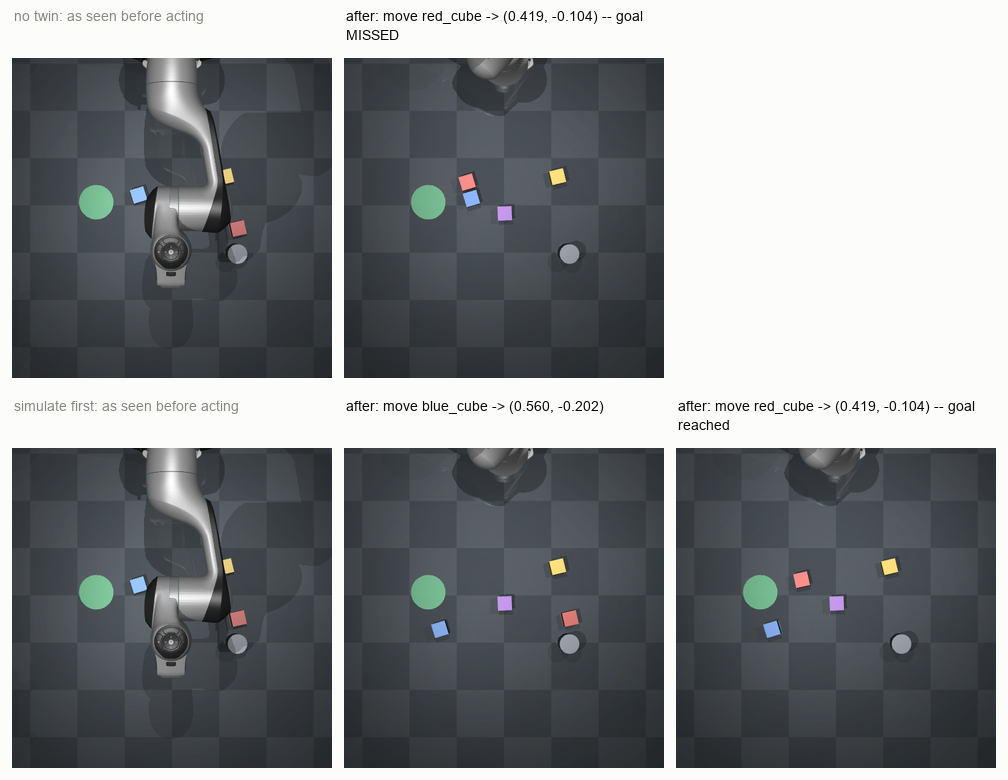
\includegraphics[width=\linewidth]{s4_loop.png}
\caption{One episode, run twice. The instruction is \emph{``put the red cube
where the blue cube is''}, and the destination is occupied. \textbf{Top:} with no
twin, the robot executes the obvious one-step plan --- pick the red cube, place
it on the blue cube's spot --- and the goal is missed, because the spot is not
free. \textbf{Bottom:} the same plan is rolled out in the twin first, predicted
to fail, and repaired into \texttt{clear-then-place}: move the blocker, then
place. Two simulated rollouts, then one execution. This is the repair that
carries the effect in Table~\ref{tab:repairs}.}
\label{fig:demo}
\end{figure}

Figure~\ref{fig:demo} shows the mechanism on a single episode before the rates.
Table~\ref{tab:headline} gives the three arms and Table~\ref{tab:paired} the
paired comparisons. The loop lifts clean success by
$8.4$ points in the open regime and $11.0$ in clutter, rescuing
\numPairedLoopDirectOpenResc\ episodes and breaking
\numPairedLoopDirectOpenBroke\ ($p = \numPairedLoopDirectOpenP$) and
\numPairedLoopDirectClutteredResc/\numPairedLoopDirectClutteredBroke\
($p = \numPairedLoopDirectClutteredP$) respectively.

The gain lands where the benchmark predicted the headroom was.
Occupied-destination tasks --- \emph{put X where Y is}, which cannot be completed
by a single pick-and-place --- rise from \numDirectOpenOcc\% to \numLoopOpenOcc\%
and from \numDirectClutOcc\% to \numLoopClutOcc\%. Table~\ref{tab:repairs} shows
why: the responsible repair is \texttt{clear-then-place}, the only one that
changes the \emph{length} of the plan, chosen in \numRepairClearthenplaceOpenN\
and \numRepairClearthenplaceClutN\ episodes and succeeding in
\numRepairClearthenplaceOpen\% and \numRepairClearthenplaceClut\% of them.

It is cheap. The loop costs a mean of \numLoopOpenSims--\numLoopClutSims\
simulated rollouts per episode and takes wall-clock from \numDirectOpenSecs\,s to
\numLoopOpenSecs\,s (open) and \numDirectClutSecs\,s to \numLoopClutSecs\,s
(cluttered) --- roughly a doubling of something that was already fast. Simulating
before acting is affordable here precisely \emph{because} an episode is cheap,
which is an argument for fast simulators and not a general argument for the
method.

% generated by paper/build_tables.py -- do not edit

\begin{table*}[t]
\centering
\caption{Clean success for the three arms. \emph{Clean} means the goal predicate holds \emph{and} no object the instruction did not license moving was displaced by more than 30\,mm. Brackets are Wilson 95\% intervals; the next column is the spread of the four per-seed rates, which is wider than several of the effects this paper measures and is why every comparison in Table~\ref{tab:paired} is paired rather than rate-against-rate.}
\label{tab:headline}
\small
\begin{tabular}{lrlllrr}
\toprule
arm & $n$ & clean success (\%) & per-seed & \emph{where Y is} (\%) & rollouts & s/ep. \\
\midrule
\multicolumn{7}{l}{\itshape open regime (3 cubes, 85\,mm minimum separation)} \\
direct (no twin) & 300 & 88.3 \ci{84.2}{91.5} & 81.3--92.0 & 66.7 \ci{57.2}{75.0} & 0.00 & 0.33 \\
loop, mis-specified twin & 300 & 96.7 \ci{94.0}{98.2} & 89.3--100.0 & 90.5 \ci{83.4}{94.7} & 1.20 & 0.55 \\
loop, exact-physics twin & 300 & 95.7 \ci{92.7}{97.5} & 93.3--97.3 & 87.6 \ci{80.0}{92.6} & 1.17 & 0.53 \\
\multicolumn{7}{l}{\itshape cluttered regime (5 cubes, 62\,mm minimum separation)} \\
direct (no twin) & 300 & 79.3 \ci{74.4}{83.5} & 76.0--82.7 & 55.6 \ci{46.9}{64.1} & 0.00 & 0.38 \\
loop, mis-specified twin & 300 & 90.3 \ci{86.5}{93.2} & 86.7--93.3 & 80.6 \ci{72.8}{86.6} & 1.28 & 0.77 \\
loop, exact-physics twin & 300 & 85.3 \ci{80.9}{88.9} & 81.3--89.3 & 68.5 \ci{59.9}{76.1} & 1.23 & 0.74 \\
\bottomrule
\end{tabular}
\end{table*}

\begin{table}[t]
\centering
\caption{Paired comparisons. Every arm ran the same layouts with the same instructions under the same seeds, so each episode is a matched pair and the comparison reduces to the episodes where the two arms disagreed. \emph{rescued} is episodes the first arm cleaned that the second failed; $p$ is McNemar's exact test on the discordant pairs.}
\label{tab:paired}
\small
\begin{tabular}{llrrrrl}
\toprule
comparison & regime & $n$ & rescued & broke & net & $p$ \\
\midrule
loop vs.\ direct & open & 300 & 25 & 0 & $+25$ & $6\times 10^{-8}$ \\
loop, exact-physics vs.\ loop & open & 300 & 3 & 6 & $-3$ & $0.508$ \\
loop vs.\ direct & cluttered & 300 & 34 & 1 & $+33$ & $2\times 10^{-9}$ \\
loop, exact-physics vs.\ loop & cluttered & 300 & 1 & 16 & $-15$ & $0.0003$ \\
\bottomrule
\end{tabular}
\end{table}

\begin{table}[t]
\centering
\caption{Three judges of the same 1{,}800 episodes, scored against the simulator's own goal predicate. The skill knows only that it grasped, carried and released; the twin predicts before acting; the camera looks afterwards. Only the false-positive column matters operationally --- it is the error a system acts on, and it is the only column that separates them: recall is near-identical because all three judges rarely reject an episode that was in fact clean. The twin's row covers the 1{,}200 episodes of the two loop arms.}
\label{tab:judges}
\small
\begin{tabular}{lrrlrr}
\toprule
judge & success calls & wrong & precision (\%) & recall (\%) & missed \\
\midrule
the skill, from inside the action & 1{,}693 & 94 & 94.4 \ci{93.3}{95.4} & 99.5 & 8 \\
the twin, before acting & 1{,}181 & 83 & 93.0 \ci{91.4}{94.3} & 99.5 & 6 \\
the camera, from one photograph & 1{,}599 & 0 & 100.0 \ci{99.8}{100.0} & 99.5 & 8 \\
\bottomrule
\end{tabular}
\end{table}

\begin{table}[t]
\centering
\caption{Failure taxonomy over all 1{,}800 episodes, by first cause. The two rows the loop was built to attack are the top two: an episode where the skill reported success and the goal was not met, and one where the goal was met by disturbing protected objects. Rows below them are ordinary skill failures, which the loop repairs only incidentally.}
\label{tab:taxonomy}
\small
\begin{tabular}{lrrrrrr}
\toprule
first cause & \multicolumn{3}{c}{open} & \multicolumn{3}{c}{cluttered} \\
\midrule
 & dir. & loop & exact & dir. & loop & exact \\
skill succeeded, goal unmet & 21 & 7 & 8 & 26 & 12 & 20 \\
released $>$50\,mm from target & 14 & 3 & 5 & 22 & 8 & 12 \\
lost the object carrying it & \textendash & \textendash & \textendash & 7 & 6 & 8 \\
fingers closed on nothing & \textendash & \textendash & \textendash & 5 & 3 & 3 \\
slipped out on the lift & \textendash & \textendash & \textendash & 2 & \textendash & 1 \\
\midrule
\textbf{total failures} & \textbf{35} & \textbf{10} & \textbf{13} & \textbf{62} & \textbf{29} & \textbf{44} \\
\bottomrule
\end{tabular}
\\[2pt]\footnotesize\raggedright dir.\ = direct, exact = loop with the exact-physics twin.
\end{table}

\begin{table}[t]
\centering
\caption{Selective autonomy, for free. A plan the twin never endorsed within its budget is still executed here, but flagged. The flag is the loop's own estimate that it is about to do something it could not verify, and episodes carrying it fail far more often --- which is what makes it usable as a request for help rather than as a label after the fact.}
\label{tab:selective}
\small
\begin{tabular}{llrlrl}
\toprule
arm & regime & coverage (\%) & clean $\mid$ endorsed (\%) & $n$ flagged & clean $\mid$ flagged (\%) \\
\midrule
loop, mis-specified twin & open & 100.0 & 96.7 \ci{94.0}{98.2} & 0 & \textendash \\
loop, exact-physics twin & open & 100.0 & 95.7 \ci{92.7}{97.5} & 0 & \textendash \\
loop, mis-specified twin & cluttered & 96.3 & 92.4 \ci{88.7}{94.9} & 11 & 36.4 \ci{15.2}{64.6} \\
loop, exact-physics twin & cluttered & 97.3 & 87.0 \ci{82.6}{90.4} & 8 & 25.0 \ci{7.1}{59.1} \\
\bottomrule
\end{tabular}
\end{table}

\begin{table*}[t]
\centering
\caption{Re-scoring every episode at tighter collateral thresholds. The 30\,mm rule used throughout never binds in these runs --- no episode met its goal and failed on displacement, and the largest displacement seen anywhere was \numCollateralMax\,mm --- so the rule as stated is untested by this experiment. Tightening it to 10\,mm costs both arms several points and leaves the paired result intact, which is the claim that needed checking.}
\label{tab:collateral}
\small
\begin{tabular}{rrrllrrll}
\toprule
$\tau$ (mm) & \multicolumn{4}{c}{open} & \multicolumn{4}{c}{cluttered} \\
\midrule
 & direct & loop & net & $p$ & direct & loop & net & $p$ \\
10 & 88.0 & 96.3 & +25/$-$0 & $6\times 10^{-8}$ & 76.7 & 86.7 & +31/$-$1 & $2\times 10^{-8}$ \\
15 & 88.3 & 96.7 & +25/$-$0 & $6\times 10^{-8}$ & 77.3 & 87.7 & +32/$-$1 & $8\times 10^{-9}$ \\
20 & 88.3 & 96.7 & +25/$-$0 & $6\times 10^{-8}$ & 78.0 & 88.7 & +33/$-$1 & $4\times 10^{-9}$ \\
30 & 88.3 & 96.7 & +25/$-$0 & $6\times 10^{-8}$ & 79.3 & 90.3 & +34/$-$1 & $2\times 10^{-9}$ \\
50 & 88.3 & 96.7 & +25/$-$0 & $6\times 10^{-8}$ & 79.3 & 90.3 & +34/$-$1 & $2\times 10^{-9}$ \\
\bottomrule
\end{tabular}
\\[2pt]\footnotesize\raggedright $\tau$ is the displacement a protected object is allowed. Rates are clean success (\%); \emph{net} is rescued/broke for loop against direct, paired per episode.
\end{table*}

\begin{table}[t]
\centering
\caption{Which plan the loop executed, and how it fared. \texttt{direct} is the one-step plan the baseline would also have run; the rest are repairs the twin demanded. \texttt{clear-then-place} is the only repair that changes the \emph{length} of the plan, and it carries the effect.}
\label{tab:repairs}
\small
\begin{tabular}{llrrl}
\toprule
plan executed & regime & $n$ & share (\%) & clean success (\%) \\
\midrule
direct & open & 239 & 79.7 & 95.8 \ci{92.5}{97.7} \\
clear-then-place & open & 61 & 20.3 & 100.0 \ci{94.1}{100.0} \\
direct & cluttered & 236 & 78.7 & 89.8 \ci{85.3}{93.1} \\
clear-then-place & cluttered & 59 & 19.7 & 94.9 \ci{86.1}{98.3} \\
turn-wrist & cluttered & 5 & 1.7 & 60.0 \ci{23.1}{88.2} \\
\bottomrule
\end{tabular}
\end{table}

\begin{table}[t]
\centering
\caption{Crossing the twin's two kinds of ignorance: wrong physics, and blindness to which way a cube is turned. The two are \emph{substitutes} --- fixing either lifts the worst cell about five points, and fixing both lifts it the same five points and no more. \emph{false confidence} is the share of episodes the twin predicted clean and were not, the error the system acts on.}
\label{tab:factorial}
\small
\begin{tabular}{lrlrrrr}
\toprule
twin & $n$ & clean success (\%) & \emph{where Y is} & twin agreed & false conf. & two-step \\
\midrule
direct (no twin) & 300 & 79.3 \ci{74.4}{83.5} & 55.6 & \textendash & \textendash & 0.0 \\
exact physics, yaw unseen & 300 & 85.3 \ci{80.9}{88.9} & 68.5 & 86.7 & 12.7 & 17.0 \\
exact physics, yaw known & 300 & 90.7 \ci{86.8}{93.5} & 81.5 & 93.0 & 6.3 & 18.7 \\
mis-specified, yaw unseen & 300 & 90.3 \ci{86.5}{93.2} & 80.6 & 91.3 & 7.3 & 19.7 \\
mis-specified, yaw known & 300 & 90.3 \ci{86.5}{93.2} & 79.8 & 94.0 & 5.7 & 18.3 \\
\bottomrule
\end{tabular}
\\[2pt]\footnotesize\raggedright Cluttered regime throughout, 300 episodes per cell, identical layouts and instructions across cells. Paired tests against the worst cell are in the text.
\end{table}

\begin{table*}[t]
\centering
\caption{Mis-specification swept through zero as a \emph{signed} magnitude along one direction in log-parameter space, so that $-1$ is the exact mirror of $+1$: where the positive twin believes cubes are heavier and more slippery than they are, the negative one believes they are lighter and grippier. \emph{useful} and \emph{accurate} come from two separate runs on purpose --- accuracy is measured on one fixed plan that no twin chose, because a twin scored on the plan it selected is being scored on its own caution.}
\label{tab:sweep}
\small
\begin{tabular}{rrlrlrrl}
\toprule
$k$ & $\lVert e\rVert$ & useful: clean (\%) & \emph{where Y is} & accurate (\%) & false conf. & pred.\ clean & paired vs.\ $k{=}0$ \\
\midrule
$-3.0$ & 0.66 & 84.3 \ci{79.8}{88.0} & 66.1 & 83.3 \ci{78.7}{87.1} & 13.0 & 88.7 & +8/$-$11 ($0.648$) \\
$-2.0$ & 0.44 & 86.7 \ci{82.4}{90.1} & 71.8 & 84.0 \ci{79.4}{87.7} & 10.3 & 84.0 & +11/$-$7 ($0.481$) \\
$-1.0$ & 0.22 & 88.3 \ci{84.2}{91.5} & 75.8 & 81.0 \ci{76.2}{85.0} & 9.0 & 78.3 & +14/$-$5 ($0.064$) \\
$-0.5$ & 0.11 & 87.3 \ci{83.1}{90.6} & 73.4 & 79.0 \ci{74.0}{83.2} & 10.7 & 79.7 & +9/$-$3 ($0.146$) \\
$+0.0$ & 0.00 & 85.3 \ci{80.9}{88.9} & 68.5 & 78.0 \ci{73.0}{82.3} & 12.0 & 81.3 & \textendash \\
$+0.5$ & 0.11 & 87.0 \ci{82.7}{90.3} & 72.6 & 77.3 \ci{72.3}{81.7} & 10.3 & 77.3 & +8/$-$3 ($0.227$) \\
$+1.0$ & 0.22 & 90.3 \ci{86.5}{93.2} & 80.6 & 84.0 \ci{79.4}{87.7} & 7.0 & 77.3 & +16/$-$1 ($0.0003$) \\
$+2.0$ & 0.44 & 89.0 \ci{85.0}{92.1} & 77.4 & 84.7 \ci{80.2}{88.3} & 7.7 & 79.3 & +18/$-$7 ($0.043$) \\
$+3.0$ & 0.66 & 90.0 \ci{86.1}{92.9} & 78.2 & 81.3 \ci{76.5}{85.3} & 7.3 & 75.3 & +23/$-$9 ($0.020$) \\
\bottomrule
\end{tabular}
\\[2pt]\footnotesize\raggedright $k$ is in units of the mis-specification the loop was built with; $\lVert e\rVert$ is the resulting distance from the truth in log-parameter space. The fixed plan actually succeeded \numFixedActual\% of the time, so a twin predicting \emph{clean} far above that figure is right by agreeing with the common case rather than by discriminating.
\end{table*}

\begin{table}[t]
\centering
\caption{What the data pins down against what the task can feel, over the same three parameters in the same units of log-parameter error. The top two are swapped: a push constrains friction roughly three times better than mass, while the task is half again more sensitive to mass than to friction. Joint damping is the sharper case --- comfortably identifiable, and worth nothing.}
\label{tab:alignment}
\small
\begin{tabular}{lrrrr}
\toprule
parameter & identification ($\sigma$ / unit) & task (points / unit) & clean at $+1$ & clean at $-1$ \\
\midrule
cube friction & 174.0 & 6.8 & 86.5 & 83.5 \\
cube mass & 65.6 & 9.1 & 88.5 & 84.5 \\
joint damping & 29.5 & 0.0 & 85.5 & 85.5 \\
\bottomrule
\end{tabular}
\\[2pt]\footnotesize\raggedright Identification sensitivity is the residual change per unit log-parameter error, referenced to sensor noise ($\numSigmaCube$\,mm on cube position, $\numSigmaJoint$\,mrad on joint angle). As unit vectors the two columns sit $\numAlignAngle^\circ$ apart (cosine $\numAlignCos$).
\end{table}


\subsection{Who can tell that something went wrong?}
\label{sec:judges}

Table~\ref{tab:judges} scores three judges of the same 1{,}800 episodes against
the simulator's own goal predicate. The skill reported success on
\numJudgeSkillSaid\ episodes and was wrong \numJudgeSkillWrong\ times. It is not
lying: it grasped, carried and released, and from inside the action that is
indistinguishable from success. The camera verifier made \numJudgeCameraSaid\
success calls and \numJudgeCameraWrong\ of them was wrong --- a precision of
\numJudgeCameraPrec\% with a Wilson lower bound of \numJudgeCameraPrecLo\%. Its
only errors run the other way: \numJudgeCameraMiss\ episodes it called failures
that were in fact clean, where a $\sim$3\,mm position estimate fell on the wrong
side of a tolerance. The verdict \emph{unsure} never fired in these runs.

Two details are worth more than the headline. First, the skill's
\numJudgeSkillMiss\ conservative errors and the camera's \numJudgeCameraMiss\ are
\emph{disjoint sets of episodes}: the two judges do not merely differ in
threshold, they fail on different things, which is the argument for keeping both
rather than replacing one. Second, the twin --- judging before the fact rather
than after --- sits between them at \numJudgeTwinPrec\% precision over
\numJudgeTwinSaid\ calls. Prediction is harder than observation, which is the
expected ordering and a sanity check that the verifier is not accidentally
reading the same signal the predictor does.

\subsection{Selective autonomy, for free}
\label{sec:selective}

The loop returns a plan even when the twin never endorsed one within its budget,
flagged \texttt{confident = False}. That flag is the system's own estimate that
it is about to do something it could not verify. Evaluated as an abstention
signal in the sense of selective classification
\citep{elyaniv2010foundations,geifman2017selective},
Table~\ref{tab:selective} shows it separates two very different populations:
pooled over both loop arms and both regimes, endorsed episodes are clean
\numSelPoolEnd\% \ci{\numSelPoolEndLo}{\numSelPoolEndHi} of the time, while the
\numSelPoolNUn\ flagged episodes are clean \numSelPoolUn\%
\ci{\numSelPoolUnLo}{\numSelPoolUnHi}. Coverage is \numSelPoolCov\%.

The flag is a hard endorsement rather than a probability, so none of the
calibration machinery developed for confident classifiers
\citep{guo2017calibration} applies directly --- there is one operating point and
we report it. The intervals do not overlap, but the flagged population is small and its
interval is correspondingly wide, so the honest claim is the ordering and not the
point estimate. The flag never fires at all in the open regime, which is
consistent with it tracking genuine difficulty rather than firing at random. A
system that can say \emph{I could not check this one} before acting can ask for
help; one that cannot tell the difference cannot, and the difference costs
nothing extra to compute --- it is a by-product of the budget the loop already
spends.

\subsection{The factorial: two ignorances, and which one dominates}
\label{sec:factorial}

The twin is wrong in two separable ways, and the first reading of the loop
experiment ---
that accuracy is simply the wrong axis --- turned out to be too broad.
Table~\ref{tab:factorial} crosses them. With exact physics and unseen
orientation the loop reaches \numFacExactBlind\%; telling it the orientation
lifts that to \numFacExactSeen\%; leaving the orientation unseen but
mis-specifying the physics lifts it to \numFacWrongBlind\%; doing both gives
\numFacWrongSeen\%.

The two ignorances are \textbf{substitutes, not additive}. Fixing either lifts
the worst cell about five points. Fixing both lifts it the same five points and
no more. Paired against the worst cell, exact/seen rescued
\numFacPairedExactphysicsyawknoResc\ and broke
\numFacPairedExactphysicsyawknoBroke\ ($p = \numFacPairedExactphysicsyawknoP$),
mis-specified/unseen rescued \numFacPairedMisspecifiedyawunsResc\ and broke
\numFacPairedMisspecifiedyawunsBroke\ ($p = \numFacPairedMisspecifiedyawunsP$).

The mechanism follows. Every cube in these layouts is turned by up to
$23^\circ$. A twin that is exactly right about mass, friction and damping while
believing every cube is square to the table simulates a grasp that is not the
grasp the robot will attempt, faithfully, and reports that it works --- an
\emph{optimistic} error. Parameter error in the pessimistic direction cancels
part of that optimism. It is worth exactly as much as seeing the orientation, and
no more, which is why the four cells saturate at the same place.

A twin with deliberately wrong physics and correct geometry also \emph{predicts}
better than one with correct physics and wrong geometry ---
\numFacWrongSeenAgree\% agreement against \numFacExactBlindAgree\%, with false
confidence \numFacWrongSeenFalse\% against \numFacExactBlindFalse\%. For this
task, knowing where things are and how they sit is worth more than knowing what
they are made of. The share of episodes choosing the two-step plan barely moves
across the four cells (\numFacExactBlindTwoStep--\numFacWrongBlindTwoStep\%),
which narrows the mechanism: the plan \emph{mix} is not what separates the arms,
it is which one-step plans get endorsed.

\subsection{The sweep: fidelity is not monotone in usefulness}
\label{sec:sweep}

\begin{figure}[t]
\centering
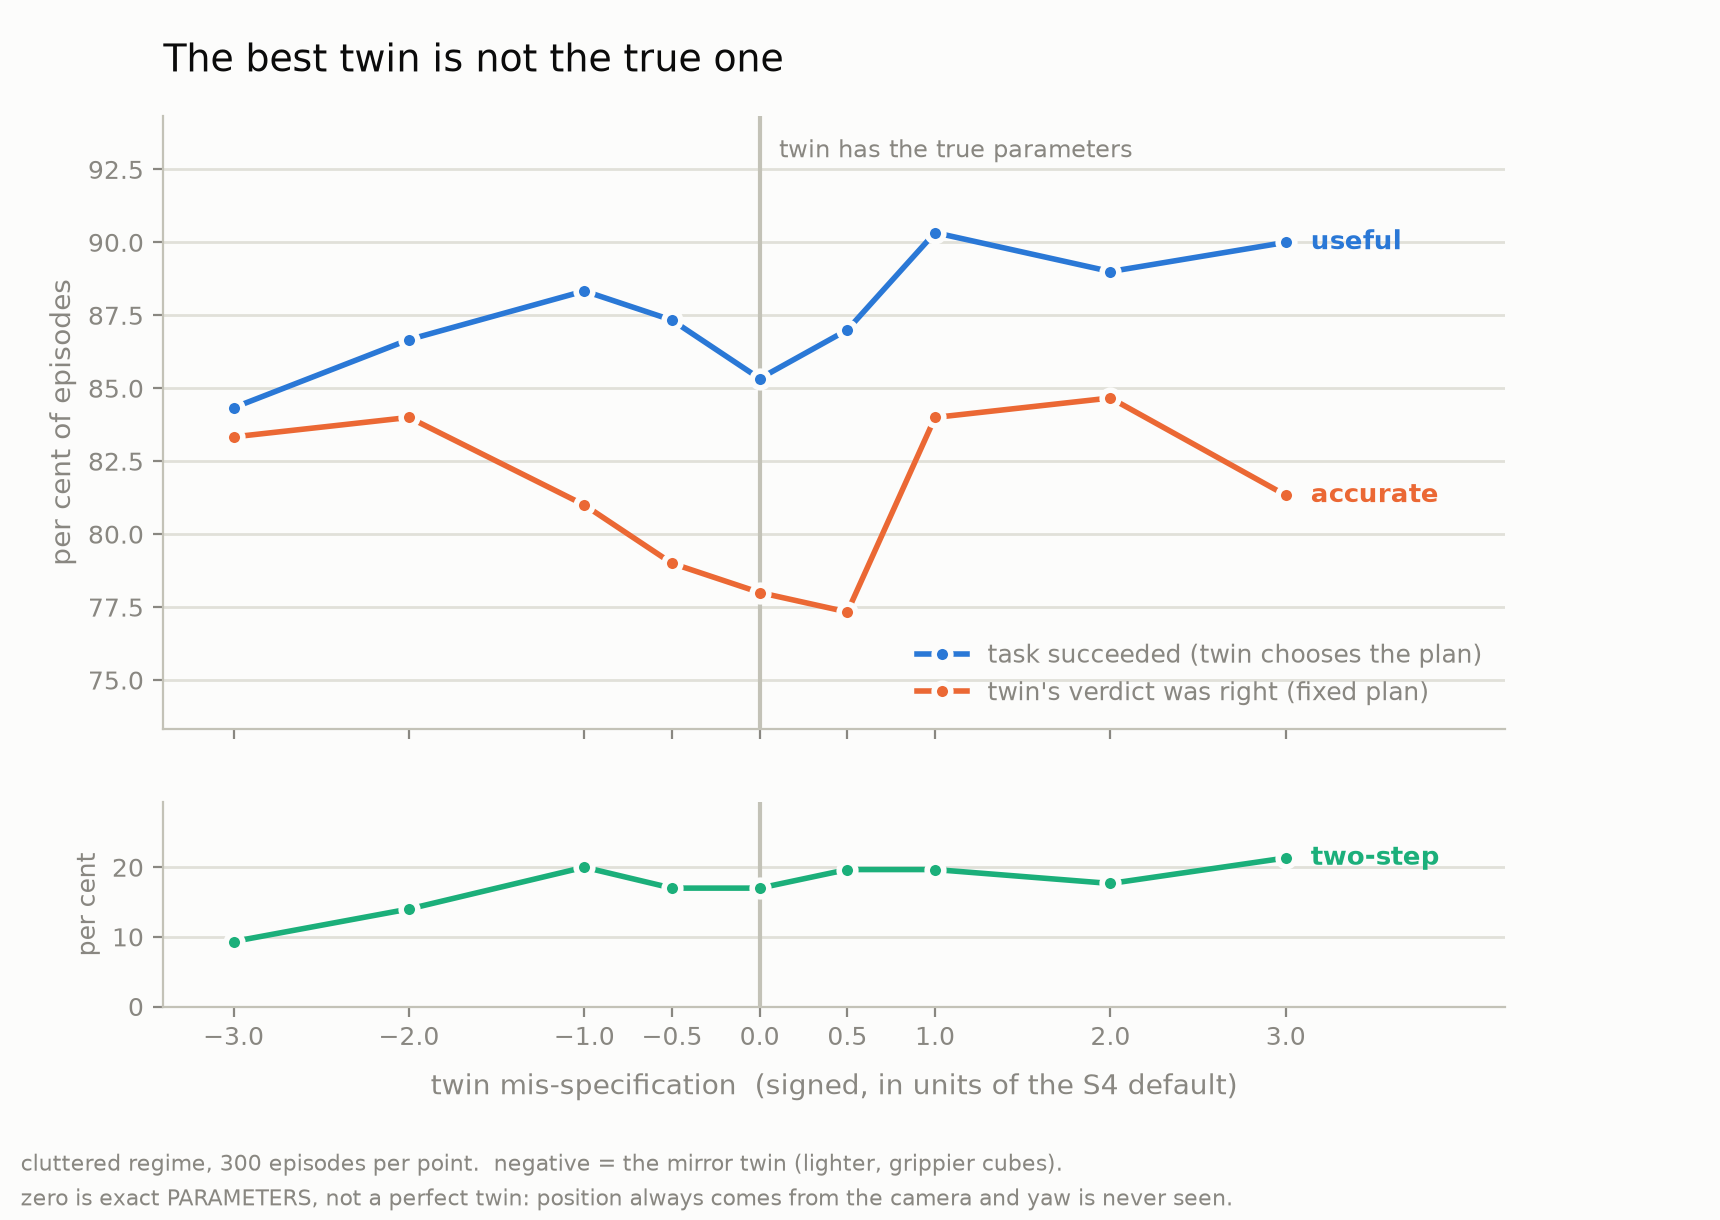
\includegraphics[width=\linewidth]{s5_fidelity.png}
\caption{Both curves bottom out at the true parameters. Blue is task success
when the twin is free to choose and repair its own plan; orange is how often the
twin's verdict was right about a plan it did \emph{not} choose, measured in a
separate run so that plan selection cannot inflate it. Negative $k$ is the
mirror twin --- lighter, grippier --- and $+1$ is the mis-specification the loop
was originally built with.}
\label{fig:sweep}
\end{figure}

Table~\ref{tab:sweep} and Figure~\ref{fig:sweep} sweep $k$ from $-3$ to $+3$.
\textbf{The twin holding the plant's true parameters is the minimum of both
curves.} It is neither the most useful --- \numSweepZero\%
\ci{\numSweepZeroLo}{\numSweepZeroHi} against \numSweepPlusOne\%
\ci{\numSweepPlusOneLo}{\numSweepPlusOneHi} at $k=+1$ --- nor the most accurate,
\numSweepZeroAcc\% against \numSweepPlusTwoAcc\% at $k=+2$. Paired against
$k=0$, the $+1$ twin rescued \numSweepPlusOneResc\ episodes and broke
\numSweepPlusOneBroke\ ($p = \numSweepPlusOneP$); $+2$ and $+3$ are also
significant ($p = \numSweepPlusTwoP$, $p = \numSweepPlusThreeP$). On the mirror
side only $k=-1$ approaches it (net $+9$, $p = \numSweepMinusOneP$), and $k=-3$
is the worst arm in the sweep.

The asymmetry is the point. If both signs helped equally, the explanation would
be that \emph{disagreement} is what helps --- the ensemble argument
\citep{mordatch2015ensemble} at $n=1$. They do not. Pessimism helps and optimism
does not, which is what the factorial predicts: there is a specific optimistic
bias in the twin, caused by unseen orientation, and only error pointing the other
way cancels it.

\subsection{Accuracy, measured on a plan the twin did not choose}
\label{sec:fixedplan}

The most instructive comparison in Table~\ref{tab:sweep} is $k=-3$ against
$k=+1$. They are indistinguishable on overall agreement --- \numSweepMinusThreeAcc\%
and \numSweepPlusOneAcc\% --- and they are the worst and the best arms for task
success (\numSweepMinusThree\% and \numSweepPlusOne\%).

The bottom rows say why. The fixed plan actually succeeded \numFixedActual\% of
the time. The optimistic twin at $k=-3$ predicts a clean outcome
\numSweepMinusThreePred\% of the time: it is right often because most plans do
work, not because it can tell which ones will not. Its false confidence is the
highest in the sweep, \numSweepMinusThreeFalse\%, nearly double the
\numSweepPlusOneFalse\% of the $+1$ twin. False confidence is the error a system
\emph{acts on}; a false alarm merely costs a repair.

So the slogan from the loop experiment --- the twin's job is not to be accurate
--- survives, but needs its second half: \textbf{the twin's job is to be right
about the failures}. A twin scored on overall agreement can buy a good number by
saying yes to everything, and that twin is the worst one to plan with. This is
the same structure as objective mismatch \citep{lambert2020objective}, sharpened
to a statement about \emph{which} errors a planning model is allowed to make.

\subsection{Identification against task sensitivity}
\label{sec:alignment}

\begin{figure}[t]
\centering
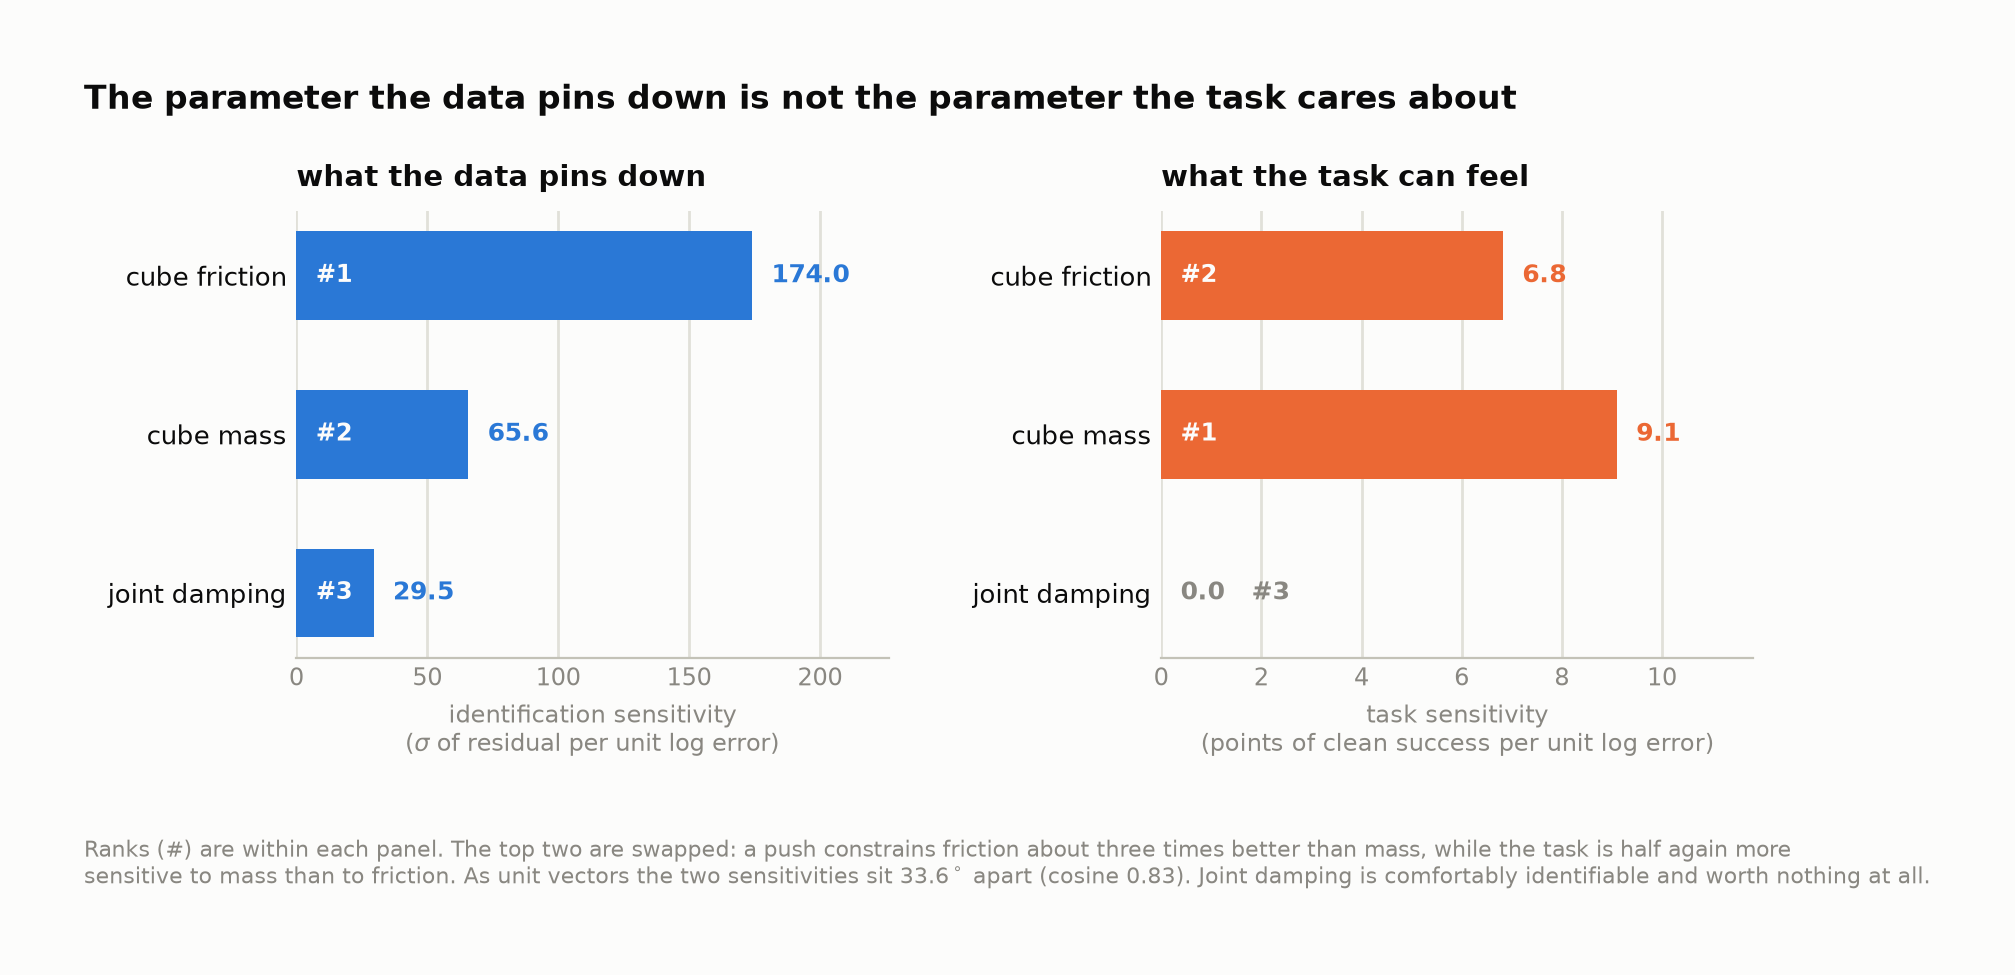
\includegraphics[width=\linewidth]{s5_alignment.png}
\caption{What a scripted push pins down, against what the task can feel, over
the same three parameters in the same units of log-parameter error. The top two
ranks are swapped, and joint damping --- comfortably identifiable --- is worth
nothing at all.}
\label{fig:alignment}
\end{figure}

Identification uses a scripted push, logging what the camera and joint encoders
would see and finite-differencing the noise-referenced residual against
log-parameters. A push rather than a pick, deliberately: a grasp is a discrete
event whose outcome flips with parameters, so the residual jumps and a finite
difference across the jump measures the jump. The residual is exactly
$0.000\sigma$ at the true parameters, which is the check that the harness is
sound --- every nonzero residual thereafter is a real effect and not harness
noise.

Table~\ref{tab:alignment} and Figure~\ref{fig:alignment} put that beside the
task's own sensitivity. The push constrains friction
($\numAlignCubefrictionSigma\sigma$ per unit log error) nearly three times better
than mass ($\numAlignCubemassSigma\sigma$); the task is half again more sensitive
to mass ($\numAlignCubemassTask$ points) than to friction
($\numAlignCubefrictionTask$ points). \textbf{The top two are swapped.} As unit
vectors the two sensitivities sit $\numAlignAngle^\circ$ apart (cosine
$\numAlignCos$) --- not orthogonal, but far enough that optimising one is not
optimising the other, and far enough that the \emph{ordering} a practitioner
would act on is reversed.

Joint damping is the sharper case. It is comfortably identifiable at
$\numAlignJointdampingSigma\sigma$ per unit log error, nothing like a null
direction. And it is worth nothing: mis-specifying it by $\pm1$ gives
\numAlignJointdampingUp\% either way against a baseline of \numSweepZero\%,
identical to three significant figures in every column we measured. A perfectly
well-posed parameter that the task cannot feel.

The practical consequence is a reordering of effort. Spending an identification
budget where the data is most informative would spend it on friction and damping.
What would actually move this system is mass --- and, well ahead of any of them,
the cube orientation the camera never reports, which is not a physics parameter
at all.

\subsection{Sensitivity to the scoring constant}
\label{sec:collateral}

Defect~\defect{D6} is that the 30\,mm collateral rule never binds in these runs.
Table~\ref{tab:collateral} re-scores every episode at tighter thresholds.
Tightening to $\tau = 10$\,mm costs the cluttered arms about three points each
(direct \numTauThirtyClutDirect\% $\to$ \numTauTenClutDirect\%, loop
\numTauThirtyClutLoop\% $\to$ \numTauTenClutLoop\%) and leaves the paired result
intact: \numTauTenClutResc\ rescued, \numTauTenClutBroke\ broken,
$p = \numTauTenClutP$. The headline conclusion does not depend on where the line
is drawn. What does remain untested is the rule's intended function --- ruling out
the bulldozing strategy --- since in these particular runs no arm attempted it.

\section{Discussion}

Three claims survive the experiments, and they are worth separating from each
other because they are usually run together.

\paragraph{A planning model should be biased, not merely accurate.}
The useful twin here is not the one closest to the plant. It is the one whose
error points in the direction that cancels the system's dominant unmodelled
optimism. That is a design instruction, not a curiosity: if you know which way
your model's unmodelled state biases it, you should mis-specify its parameters
the other way. The ensemble literature \citep{mordatch2015ensemble,
rajeswaran2017epopt} gets robustness by averaging over perturbations, which is
strictly more expensive and, because it averages, cannot exploit a known sign.

\paragraph{Score a model on the errors you will act on.}
Overall agreement rewards a model for agreeing with the base rate. The $k=-3$
twin demonstrates the failure mode concretely: equal agreement to the best arm,
worst task performance, highest false confidence. Any fidelity metric used to
decide whether a twin is good enough should be asymmetric, because the
consequences are.

\paragraph{Spend identification effort where the task is sensitive, not where
the data is informative.} Classical experiment design optimises the conditioning
of the identification problem \citep{gautier1992exciting,pukelsheim1993optimal}.
That is the right objective only if identifiability and task sensitivity are
aligned, and on this system they are $\numAlignAngle^\circ$ apart with their top
two ranks swapped. The strongest version of the point is joint damping: cleanly
identifiable, and worth zero.

Underneath all three is the same observation from a different side. Effort spent
on the twin's \emph{physics} was worth less than effort spent on the
\emph{perception feeding it}. The twin's dominant error was never a parameter it
had wrong; it was a state variable the camera does not report. That is why the
next step for this system is a vision-language model asked for cube orientation
rather than for instruction grounding --- a target the experiments chose, not one
the plan started with.

\section{Limitations and threats to validity}
\label{sec:limits}

\paragraph{Simulation only.} There is no hardware anywhere in this work. The
central result is about a twin of a simulator, where exactness is achievable and
therefore measurable; on hardware it is not. Whether the shape of
Figure~\ref{fig:sweep} survives the transfer is untested, and it is the first
thing a follow-up should check.

\paragraph{Determinism.} MuJoCo is deterministic. Variation across episodes comes
from the layout and instruction draw, not from the physics. A plant with genuine
process noise might reward an accurate twin more, because the twin's job would
then include tracking a distribution rather than a trajectory.

\paragraph{One task family, one robot, three parameters.} All results are a Panda
on a tabletop with cubes, and the parameter space the twin is wrong in has three
dimensions. The claim that identifiability and task sensitivity are misaligned is
demonstrated, not proved general; a three-dimensional example cannot establish
how common the misalignment is.

\paragraph{Sample size and seed noise.} At $n\approx300$ an absolute rate here
carries roughly $\pm7$ points of seed noise (defect~\defect{D3}). That is larger
than several differences we report, which is why every comparison is paired and
why the absolute rates should be read as context rather than as calibrated
constants. The selective-autonomy result in particular rests on
\numSelPoolNUn\ flagged episodes and its interval is wide.

\paragraph{An untested scoring rule.} The collateral threshold never binds
(defect~\defect{D6}). Section~\ref{sec:collateral} shows the headline result is
robust to tightening it, but the rule's intended deterrent function is unexercised
by these runs.

\paragraph{Grounding is not evaluated.} References are resolved from ground truth.
This is deliberate --- it isolates the loop from the grounding problem --- but it
means the system's end-to-end performance under a real language front-end is
unmeasured.

\section{Conclusion}

We built a tabletop manipulator that simulates its plan before acting and
verifies the result afterwards, and used it to ask how good the simulation has to
be. The answer is that the question was mis-posed. The twin with the plant's true
parameters is the worst twin in a nine-point sweep, because its dominant error is
not a parameter but a state variable --- the orientation of the objects it is
about to grasp --- and parameter error in the pessimistic direction cancels the
optimism that blindness causes. Accuracy measured as overall agreement rewards a
twin for agreeing with the common case; the twin that does so carries the highest
false confidence in the sweep and is the worst one to plan with. And the
parameter a scripted push identifies best is not the parameter the task is most
sensitive to.

The practical summary for anyone building a twin into a control loop: find out
which way your unmodelled state biases your model, bias your parameters the other
way, score the model on the errors you will act on rather than on agreement, and
check that your identification budget is being spent on something the task can
feel.

The next step for this system is the one the experiments pointed at rather than
the one the plan began with: a vision-language model asked to report which way
each object is turned, repairing the twin's dominant error. Section~\ref{sec:judges}
and Section~\ref{sec:alignment} between them set the baseline it would have to
beat --- \numSigmaCube\,mm position error at 37\,ms with no learned component, and
a verifier that has yet to make a single wrong success call.

\appendix
\section{Reproduction}
\label{app:repro}

\begin{table}[h]
\centering
\small
\begin{tabular}{@{}p{4.7cm}p{9.2cm}@{}}
\toprule
produces & command \\
\midrule
Tables~\ref{tab:headline}--\ref{tab:repairs} & \texttt{python experiments/bench\_loop.py 15 5 0,1,2,3} \\
Table~\ref{tab:factorial} & \texttt{python experiments/sweep\_fidelity.py factorial 15 5 0,1,2,3} \\
Table~\ref{tab:sweep}, Fig.~\ref{fig:sweep} & \texttt{python experiments/sweep\_fidelity.py sweep 15 5 0,1,2,3} \\
Table~\ref{tab:sweep} (accuracy column) & \texttt{python experiments/sweep\_fidelity.py fixedplan 15 5 0,1,2,3} \\
Table~\ref{tab:alignment} & \texttt{python experiments/sweep\_fidelity.py directions} \ and \ \texttt{python experiments/identify\_task.py} \\
Figure~\ref{fig:demo} & \texttt{python experiments/demo\_loop.py} \\
Figure~\ref{fig:alignment} & \texttt{python experiments/plot\_alignment.py} \\
Tables~\ref{tab:taxonomy},~\ref{tab:selective},~\ref{tab:collateral} and every number in the text & \texttt{python paper/build\_tables.py} \\
the document & \texttt{make -C paper} \\
\bottomrule
\end{tabular}
\end{table}

\noindent
\texttt{build\_tables.py} is pure post-processing of the committed JSON in
\texttt{results/}; it runs in under a second and needs no simulator. The
benchmark commands re-run the episodes and take roughly 15 and 50 minutes
respectively on one Apple M5 core.

\bibliography{refs}

\end{document}
